\documentclass[a4paper, 14pt]{extarticle}

\usepackage{../latex/misc/preamble2}

\geometry{a4paper}

% Название дисциплины
\newcommand{\subject}{Физика} 

% Тип работы
% lab - для лабораторной работы 
% hw  - для домашней     работы
\newcommand{\task}{lab} 

% Номер работы
\newcommand{\taskNumber}{Ф60} 

% Название работы
\newcommand{\taskNameOne}{Проверка формулы Шокли для p-n} 
\newcommand{\taskNameTwo}{перехода и определение} 
\newcommand{\taskNameThree}{ширины запрещенной зоны германия.} 

% Имя студента
\newcommand{\studentName}{Очкин Н.В.}

% Имя преподававателя
\newcommand{\teacherName}{Применко А.Э.}

% Группа
\newcommand{\group}{ФН11-52Б}

% Вариант
\newcommand{\variant}{9}

\begin{document}

\graphicspath{ {../latex/images} } 
\normalsize

\newcommand{\printTask}{%
    \ifthenelse{\equal{\task}{lab}}{%
        лабораторной%
    }{%
        \ifthenelse{\equal{\task}{hw}}{%
            домашней%
        }{%
            Неизвестный тип задания%
        }%
    }%
}

\begin{titlepage}

    \begin{center}
        {\footnotesize \itshape Федеральное государственное бюджетное 
                       образовательное учреждение высшего образования}
    \end{center}

    \begin{minipage}[c]{0.1\textwidth}
        
\includegraphics[width=1.1\textwidth]{iconBMSTU}
    \end{minipage}
    \hfill
    \begin{minipage}[c]{0.9\textwidth}
        \centering
        \itshape
        \bfseries
        \small
        \guillemotleft Московский государственный технический университет \\
        имени Н.Э. Баумана\guillemotright \\
        (национальный исследовательский университет) \\
        (МГТУ им. Н.Э. Баумана) 
    \end{minipage}

    \vspace{0.5cm}
    \noindent\rule{\textwidth}{2pt} \\

    \noindent\uline{\textbf{ФАКУЛЬТЕТ} ФУНДАМЕНТАЛЬНЫЕ НАУКИ} \\
    \vspace{-5pt} \\
    \noindent\uline{\textbf{КАФЕДРА} ВЫЧИСЛИТЕЛЬНАЯ МАТЕМАТИКА И МАТЕМАТИЧЕСКАЯ} \\
    \vspace{-5pt} \\
    \noindent\uline{ФИЗИКА (ФН11)} \\
    \vspace{-5pt} \\
    \noindent\uline{\textbf{НАПРАВЛЕНИЕ ПОДГОТОВКИ} МАТЕМАТИКА И КОМПЬЮТЕРНЫЕ} \\
    \vspace{-5pt} \\
    \noindent\uline{НАУКИ (02.03.01)} \\

    \begin{center}
        \bfseries
        \textsc{О т ч е т} \\[10pt]
        по \printTask {} работе \taskNumber
    \end{center}

    \vspace{10pt}

    \hspace{10pt} 
    \noindent \textbf{Название \printTask {} работы:} \par
    \vspace{5pt}
    \hspace{10pt} 
    \noindent \textbf{\uline{\taskNameOne}} \vspace{5pt} \\
    \null\hspace{31pt} 
    \textbf{\uline{\taskNameTwo}} \vspace{5pt} \\
    \null\hspace{31pt} 
    \textbf{\uline{\taskNameThree}}

    \vspace{10pt}

    \begin{center}
        \bfseries
        Вариант \textnumero {} \variant
    \end{center}

    \vspace{20pt}

    \hspace{10pt} 
    \noindent \textbf{Дисциплина:} \par
    \vspace{10pt}
    \hspace{10pt} 
    \noindent {\large \subject}

    \vspace{10pt}

    \begin{flushright}
        \renewcommand{\arraystretch}{3}
        \begin{tabular}{r r r}
            \multicolumn{1}{l}{Студент группы \uline{\group}} & 
            $\quad \underset{\text{(Подпись, дата)}}{\underline{\hspace{3cm}}} \quad$ & 
            \multicolumn{1}{c}{$\underset{\text{(И.О. Фамилия)}}{\uline{\textbf{\studentName}}}$} \\

            \multicolumn{1}{l}{Преподаватель} & 
            $\quad \underset{\text{(Подпись, дата)}}{\underline{\hspace{3cm}}} \quad$ & 
            \multicolumn{1}{c}{$\underset{\text{(И.О. Фамилия)}}{\uline{\textbf{\teacherName}}}$} \\
        \end{tabular}
    \end{flushright}

    \vfill

    \begin{center}
        \small
        Москва, 2024
    \end{center}
\end{titlepage}


\newgeometry{left=25mm, right=25mm, top=20mm, bottom=20mm}

\graphicspath{ {../latex/images/F60} }

% Customize section, subsection, subsubsection and paragraph styles
\titleformat{\section}
  {\normalfont\large\bfseries}{\thesection}{1em}{}

\titleformat{\subsection}
  {\normalfont\normalsize\bfseries}{\thesubsection}{1em}{}

\titleformat{\subsubsection}
  {\normalfont\small\bfseries}{\thesubsubsection}{1em}{}

\titleformat{\paragraph}
  {\small\small\bfseries}{\theparagraph}{1em}{}

% \thispagestyle{empty}

% \null\newpage

% \setcounter{tocdepth}{5}
% \setcounter{secnumdepth}{5}

% \pagenumbering{roman}

% \tableofcontents
% \newpage

% \pagenumbering{arabic}
% \setcounter{page}{1}

\setstretch{1}
\linespread{1.1}

\setlength{\parindent}{0pt}

\fontsize{14pt}{16pt}\selectfont

% \definecolor{myblue}{HTML}{0A88C2}
% \definecolor{myred}{HTML}{FF1B1C}
% \definecolor{mygreen}{HTML}{386641}

% \lstdefinestyle{mystyle}{
%     basicstyle=\ttfamily\footnotesize,
%     keywordstyle=\color{myblue},
%     stringstyle=\color{myred},
%     commentstyle=\color{green!50!black},
%     showstringspaces=false,
%     frame=leftline, 
%     framesep=10pt, 
% }

% % Set the style for Python code
% \lstset{style=mystyle, extendedchars=\true}

% --------------------------------------START--------------------------------------

\section*{Задание}\vspace{-20pt}\rule{\linewidth}{0.1mm}

\subsection*{Опыт 1}

\begin{enumerate}
    \item По результатам измерений (табл. 1) построить графическую зависимость тока диода от напряжения.
    \item Убедиться в существовании тока насыщения. Для дальнейшего расчета значение тока насыщения $I_{S}$ взять без округления из табл. 1 при обратном смещении примерно $0,15-0,20$ В.
    \item Для различных напряжений вычислить величину $\ln \left(1+I / I_{S}\right)$, результаты записать в табл. 2.
    \item На миллиметровой бумаге формата А4 построить графическую зависимость величины $\ln \left(1+I / I_{S}\right)$ от напряжения (рис. 11).
    \item В области напряжений примерно от $-0,1$ до $+0,05$ В точки должны хорошо ложиться на прямую линию, которую следует провести. Тем самым подтверждается формула Шокли (6,7).
    \item Из наклона прямой на графике находят численное значение коэффициента пропорциональности $q / k T$. Для этого на полученном графике строят треугольник, как пояснено на рис. 11, и вычисляют искомую величину по формуле $q / k T = \Delta \ln \left(1+I / I_{S}\right) / \Delta U$.
    \item Зная температуру диода $T$, получают численное значение для отношения фундаментальных физических величин $q / k$ и сравнивают его с табличным значением, равным $(q / k)_{\text{табл}} = 11590$ Кл К / Дж.
    \item Вычислить относительную погрешность измерения отношения $q / k$ в процентах, приняв за абсолютную погрешность разность между измеренным и табличным значениями.
    \item Результат измерения привести в виде $q / k = \ldots \ldots (\pm \ldots \ldots \%)$ Кл К / Дж.
\end{enumerate}

\subsection*{Опыт 2}

\begin{enumerate}
    \item Вычислить величины $T$, $1 / T$ и $\ln \left(I_{S} / I_{S O}\right)$, записать их в табл. 2. Ток насыщения при минимальной температуре $T_{0}$ обозначен $I_{S O}$ (см. раздел 6 теоретической части).
    \item По результатам измерений построить графическую зависимость величины $\ln \left(I_{S} / I_{S O}\right)$ от $1 / T$, схематически показанную на рис. 12 точками. (Примечание: ось абсцисс начинать не от нуля, а от минимального значения величины $1 / T$.) Через экспериментальные точки необходимо провести наилучшую "на глаз" прямую. Если точки мало отклоняются от проведенной прямой, то опыт подтверждает температурную зависимость (8). Значение величины $E_{g} / k$ можно получить, подставив в (10) значения $1 / T$ и $\ln \left(I_{S} / I_{S O}\right)$ для какой-либо точки, лежащей на прямой в верхней части графика. Затем вычислить значение $E_{g}$ в джоулях и электронвольтах (1 эВ = $1,61 \times 10^{-19}$ Дж, $k = 1,38 \times 10^{-23}$ Дж/К).
    \item Вычислить относительную погрешность измерения величины $E_{g}$ в процентах, приняв за абсолютную погрешность разность между измеренным и табличным значениями, $\left(E_{g}\right)_{\text{табл}} = 0,66$ эВ.
    \item Результат измерения привести в виде $E_{g} = \ldots \ldots \ldots (\pm \ldots \ldots \%)$ эВ.
\end{enumerate}

\section*{Ход выполнения работы}

\subsection*{Опыт 1}\vspace{-20pt}\rule{\linewidth}{0.1mm}

\begin{center}
    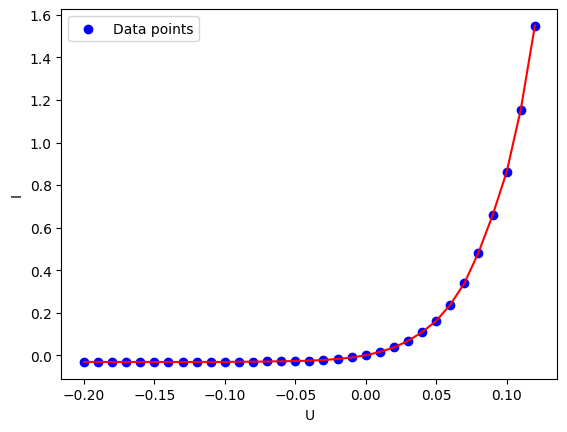
\includegraphics[width=0.9\textwidth]{1}
\end{center}

\begin{equation*}
    \text{I}_\text{S} = 0.031 \hspace{3pt} \text{мкА}
\end{equation*}

\vfill

\begin{center}
    \begin{table}[h!]
        \centering
        \begin{tabular}{|c|c|c|c|}
        \hline
        \textnumero & \text{U, В} & \text{I, мкА} & \text{ln}(\text{1 + I/}$\text{I}_\text{S}$) \\
        \hline
        1 & -0.2 & -0.031 & - \\
        2 & -0.19 & -0.031 & - \\
        3 & -0.18 & -0.031 & - \\
        4 & -0.17 & -0.031 & - \\
        5 & -0.16 & -0.031 & - \\
        6 & -0.15 & -0.031 & - \\
        7 & -0.14 & -0.031 & - \\
        8 & -0.13 & -0.031 & - \\
        9 & -0.12 & -0.031 & - \\
        10 & -0.11 & -0.031 & - \\
        11 & -0.1 & -0.031 & - \\
        12 & -0.09 & -0.03 & -3.434 \\
        13 & -0.08 & -0.03 & -3.434 \\
        14 & -0.07 & -0.029 & -2.7408 \\
        15 & -0.06 & -0.028 & -2.3354 \\
        16 & -0.05 & -0.027 & -2.0477 \\
        17 & -0.04 & -0.025 & -1.6422 \\
        18 & -0.03 & -0.022 & -1.2368 \\
        19 & -0.02 & -0.017 & -0.7949 \\
        20 & -0.01 & -0.01 & -0.3895 \\
        21 & 0.0 & 0.0 & 0.0 \\
        22 & 0.01 & 0.016 & 0.4162 \\
        23 & 0.02 & 0.037 & 0.7855 \\
        24 & 0.03 & 0.068 & 1.1611 \\
        25 & 0.04 & 0.109 & 1.5077 \\
        26 & 0.05 & 0.162 & 1.8287 \\
        27 & 0.06 & 0.238 & 2.1607 \\
        28 & 0.07 & 0.339 & 2.4795 \\
        29 & 0.08 & 0.483 & 2.8082 \\
        30 & 0.09 & 0.658 & 3.1013 \\
        31 & 0.1 & 0.862 & 3.3606 \\
        32 & 0.11 & 1.155 & 3.6444 \\
        33 & 0.12 & 1.548 & 3.9306 \\
        \hline
        \end{tabular}
    \end{table}
\end{center}

\vfill

\newpage

\begin{center}
    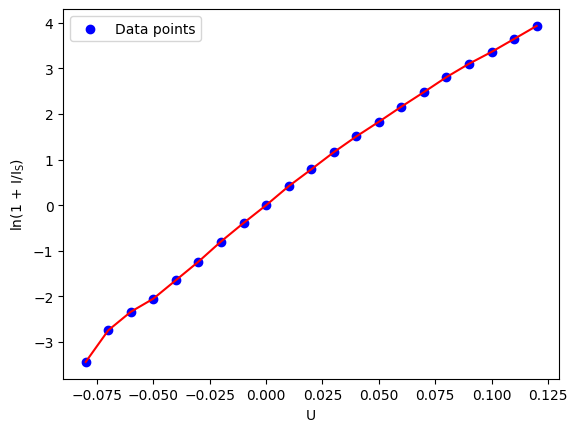
\includegraphics[width=1\textwidth]{2}
\end{center}

\begin{center}
  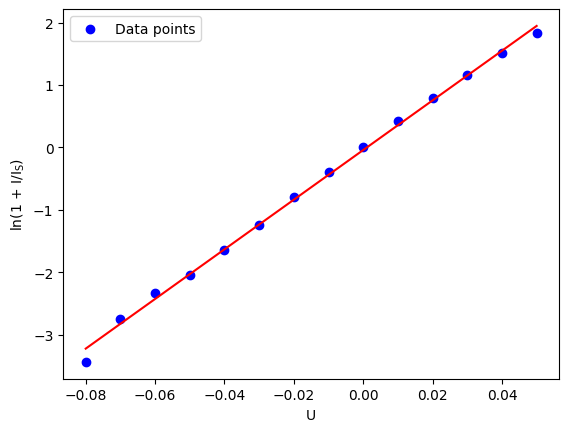
\includegraphics[width=1\textwidth]{3}
\end{center}

\begin{center}
  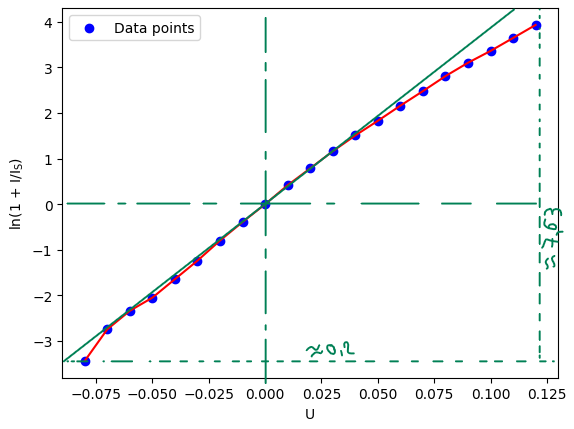
\includegraphics[width=1\textwidth]{4}
\end{center}

\begin{equation*}
  \cfrac{q}{kT} \approx \cfrac{7.63}{0.2} = 38.15
\end{equation*}

\begin{equation*}
  T = 20.2 \hspace{3pt} C^{\circ} = 293.35 K \rightarrow \cfrac{q}{k} \approx 11191 \hspace{3pt} \text{Кл К / Дж}
\end{equation*}

\begin{equation*}
  \cfrac{q}{k} = 11191 \pm 3.443 \% \hspace{3pt} \cfrac{\text{Кл } \cdot \text{ К}}{\text{Дж}}
\end{equation*}

\newpage

\subsection*{Опыт 2}\vspace{-20pt}\rule{\linewidth}{0.1mm}

\begin{center}
  \begin{table}[h!]
    \centering
    \resizebox{0.9\textwidth}{!}{ % Scale the table to the width of the text
    \setlength{\tabcolsep}{10pt}
    \begin{tabular}{cccccc}
    \toprule
    \textnumero & $t, C^{\circ}$ & $T, K$ & $\frac{1}{T}$ & $I_S$ & $\text{ln}(I_S/I_{S0})$ \\
    \midrule
    1  & 22 & 295.15 & 0.00338811 & -0.020 & 0.00000000 \\
    2  & 27 & 300.15 & 0.00333167 & -0.028 & 0.33647224 \\
    3  & 33 & 306.15 & 0.00326637 & -0.049 & 0.89608802 \\
    4  & 36 & 309.15 & 0.00323468 & -0.057 & 1.04731899 \\
    5  & 39 & 312.15 & 0.00320359 & -0.068 & 1.22377543 \\
    6  & 42 & 315.15 & 0.00317309 & -0.083 & 1.42310833 \\
    7  & 45 & 318.15 & 0.00314317 & -0.099 & 1.59938758 \\
    8  & 48 & 321.15 & 0.00311381 & -0.119 & 1.78339122 \\
    9  & 51 & 324.15 & 0.00308499 & -0.142 & 1.96009478 \\
    10 & 54 & 327.15 & 0.00305670 & -0.168 & 2.12823171 \\
    \bottomrule
    \end{tabular}
    }
    \end{table}
\end{center}

\begin{equation*}
  I_{S0} = -0.02 \text{мкА} \qquad T_0 = 295.15 \text{K}
\end{equation*}

\begin{center}
  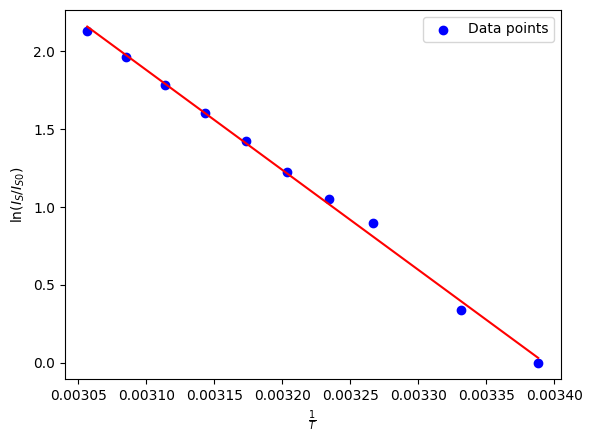
\includegraphics[width=1\textwidth]{5}
\end{center}

\begin{center}
  Возьмем T = 315.15
\end{center}

\begin{equation*}
  \cfrac{E_g}{k} = \cfrac{\text{ln}(I_S/I_{S0})}{1/T_0 - 1/T} \approx 6619 K
\end{equation*}

\begin{equation*}
  E_g = 9.13 \cdot 10^{-20} \text{Дж} \approx 0.571 \text{эВ}
\end{equation*}

\begin{equation*}
  E_g = 0.571 \pm 13.48 \hspace{3pt} \% \hspace{3pt} \text{эВ}
\end{equation*}

\end{document}